\chapter{Evaluation}
\label{cha:eva}
The analysis of the new model was performed using \textbf{Plexe} \cite{segata2014plexe}. Plexe is an extension of Veins which permits the realistic simulation of platooning (i.e., automated car-following) systems. It features realistic vehicle dynamics and several cruise control models, permitting the analysis of control systems, large-scale and mixed scenario, as well as networking protocols and cooperative maneuvers. \vskip 1em
By default, Veins comes with a scenario that simulate the traffic in the city of Erlangen, Germany, while Plexe comes with a scenario that simulate an highway where the user can choose the number of lanes, the number of nodes in the network and the platoon size. This can extremely useful since different kind of simulations can be made. Furthermore, vehicles can be dynamically inserted or deleted from the network. In the scenario used for the tuning and the evaluation of the model, the cars are inserted using a fixed speed and a random distance from the preceding vehicle. The random distance is governed by a variable with a uniform distribution between \SI{10}{\m} and \SI{50}{\m}. When a vehicle is inserted, the distance from the preceding vehicle is computed by decreasing the position of the preceding vehicle in that lane by the result of the random variable and the length of the car, after that the Cruise Control speed is set to the one specified in the initialization and the CACC constant spacing is set to the distance between the car and the preceding car in its lane. Setting the CACC constant spacing is crucial, once the vehicle joins the network, the joiner notifies the leader that it is able to join the platoon. The leader sends back a confirmation and the joiner switches to CACC, closing its gap to the predecessor to the platoon inter-car distance.
Since the inter-car distance can be different from the computed distance between the two vehicles, the joiner can have a different distance, forcing the constant spacing can avoid this issue and so the distance will remain the same unless the Cruise Control speed is changed.\vskip 1em
The exchange of messages starts as soon as the vehicles join the network and it is governed by beacons sent by each vehicle to its neighbors every \SI{0.1}{\s}.
When sending the message, the Platooning Protocol fetch the speed, acceleration and the simulation time of the sender through the TraCICommandInterface and put them into the beacon, then the beacon is encapsulated into a Unicast Message and finally sent to the lower layer.\\
When the Platooning Application of the receiver receives the message, it will check if the beacon comes from a vehicle of the same platoon, if so it will update the its information according if the beacon comes from the leader of its platoon or from a preceding vehicle of its platoon. \vskip 1em
\section{Parameters Estimation}
\label{sec:estimation}
The estimation of the parameters has been made by running three simulations with 160, 320 and 640 vehicles in the scenario, and each simulation has been repeated 10 times with different a seed for the generation of the random numbers. The parameters used in the simulations are shown in \Cref{tab:param_simulations}.
\begin{table}[H]
    \centering
    {\tabulinesep=1.2mm
    \begin{tabu}{l|l}
        \hline
        Parameter & Value  \\
        \hline
        nCars & 160,320,640    \\
        platoonSize & 4 \\
        nLanes  & 4 \\
        platoonInsertSpeed& \SI{130}{\km\per\hour} \\
        startCommunication & Time Instant \\
        startCommunicationTime & \SI{0}{\s}\\
        communicationDuration & \SI{70}{\s}\\
        statStart & \SI{50}{\s}\\
        statInterval & \SI{10}{\s}\\
        leaderSpeed & \SI{130}{\km\per\hour} \\
        \hline
    \end{tabu}}
    \caption{The parameters used during the simulations}
    \label{tab:param_simulations}
\end{table}

The recording of the simulation is set to \SI{10}{\s} since recording all the simulation would be very expensive in term of memory used to store all the information.
\Cref{fig:original} shows the Analogue Model and the Decider used during the simulations with the original model.\vskip 3em
\begin{figure}[H]
\begin{lstlisting}[frame=bt, language=XML, numbers=none]
<root>
    <AnalogueModels>
        <AnalogueModel type="SimplePathlossModel">
            <parameter name="carrierFrequency" type="double" value="5.890e+9"/>
            <parameter name="alpha" type="double" value="2.3"/>
        </AnalogueModel>
        <AnalogueModel type="GenericFading">
            <parameter name="distribution" type="string" value="gaussian"/>
            <parameter name="param1" type="double" value="2.3"/>
        </AnalogueModel>
    </AnalogueModels>
    <Decider type="Decider80211p">
        <parameter name="centerFrequency" type="double" value="5.890e9"/>
    </Decider>
</root>
\end{lstlisting}
\caption{The XML configuration of the original model.}
\label{fig:original}
\end{figure}\vskip 2em
\Cref{fig:originalmodel} shows the results of the original model with 640 vehicles. The zones where there are not data are plotted in black. The plot is done using \textbf{Python}, grouping the results by the slotted distance and the number of neighbors. The distance is divided into 40 intervals with a range of \SI{20}{\m}. As can be seen the Packet Delivery Rate decrease with the increasing of the neighbors and the distance.\vskip 1em
Only the scenario with 640 vehicles is used to compute the distance, since merging all the 30 repetitions, i.e. 10 for each scenario, would be impossible due to an high RAM usage. As can be seen in the first plot, the probability of correctly receives a frame decreases with the increase of the distance and the neighbors.\vskip 1em
The extrapolation of the parameters has been made using \textbf{R}. First of all, the data are grouped by the distance and the neighbors. Then each interval is used to fit a weighted quadratic function, where weights are given by the occurrence of each possible neighbors in the interval. In fact, there can be neighbors that have an higher number of occurrences in respect to others neighbors, so it is correct to give different weights to different occurrences. Finally, the coefficients of each interval are printed in a csv file, which is then used by the new model.\vskip 1em With this approach the new model do not need to have different probabilities for the two state, since the probability of do not correctly decode a frame due to the Nic in Tx Mode or synced with another frame is already fitted in the function. The resulting function is the following:
\begin{gather}
    y=ax^2 + bx + c
\end{gather}
where:
\begin{itemize}
    \item $a$, $b$, $c$ are the coefficients of the intervals
    \item $x$ is the neighbors;
    \item $y$ is the probability of correctly receives a frame.
\end{itemize}
\begin{figure}[H]
    \centering
    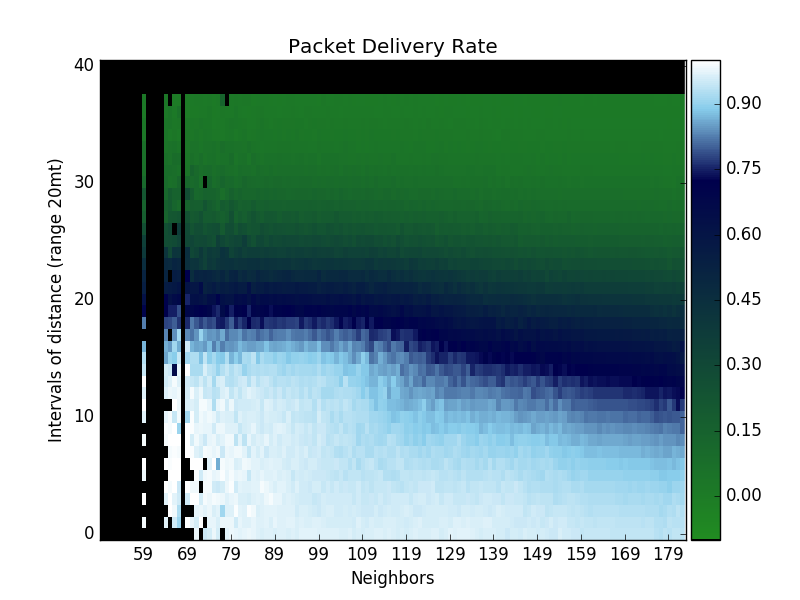
\includegraphics[width=0.8\textwidth]{fig/Original_640_plot.png}
    \caption{Packet Delivery Rate for each interval of distance and number of neighbors of the original model}
    \label{fig:originalmodel}
\end{figure}
\newpage
Once the parameters are estimated, the analysis of the two models was performed by running three simulation with 640 nodes per model. The Analogue Model and the Decider used for the new model are shown in \Cref{newmodel}.
\begin{figure}[H]
\begin{lstlisting}[frame=bt, language=XML, numbers=none]
<root>
    <AnalogueModels>
        <AnalogueModel type="ThesisAnalogueModel"></AnalogueModel>
    </AnalogueModels>
    <Decider type="ThesisDecider">
        <parameter name="centerFrequency" type="double" value="5.890e9"/>
        <parameter name="intervals" type="double" value="40"/>
        <parameter name="range" type="double" value="20"/>
        <parameter name="coefficients" type="string" value="coefficients.csv"/>
    </Decider>
</root>
\end{lstlisting}
\caption{The XML configuration of the new model.}
\label{newmodel}
\end{figure}
In order to have comparable results, the two simulations have to be dynamically equivalent. This means that at each instant the vehicles in the two simulations have to be in the same position, otherwise the two models cannot be compared. This is done by using the same seed for generating the random numbers. \vskip 1em
\section{Simulation efficiency gain}
\label{sec:gain}
The first metric analyzed is the efficiency gain of the new model with regards to the original model.
The analysis was performed by measuring the computational time while the communication between nodes is active. As described in \Cref{sec:prob}, the main problem of the original model is the computational time used during the computation of the SNR and the SINR. \vskip 1em
\subsection{Results}
\begin{table}[H]
    \centering
    {\tabulinesep=1.2mm
    \begin{tabu}{l|l l l|l}
        \hline
        Repetition & 1 & 2 & 3 & Mean \\
        \hline
           Original model &  \SI{16}{\hour} \SI{10}{\minute}  &  \SI{16}{\hour} \SI{20}{\minute}  &  \SI{16}{\hour} \SI{18}{\minute}  &  \SI{16}{\hour} \SI{16}{\minute}  \\
         New model & \SI{3}{\hour} \SI{50}{\minute} &  \SI{3}{\hour} \SI{55}{\minute}  &  \SI{3}{\hour} \SI{47}{\minute}  &  \SI{3}{\hour} \SI{51}{\minute}   \\
    \hline
        Decrease & $76\%$ & $76\%$ & $77\%$ & $76\%$ \\
        \hline
    \end{tabu}}
    \caption{Duration of the simulations}
    \label{tab:duration}
\end{table}
As can be seen from \Cref{tab:duration}, the mean duration of the new model is \SI{3}{\hour} \SI{51}{\minute}, while the original model takes on average \SI{16}{\hour} \SI{16}{\minute}. This means that there is a decrease of the $76\%$ in the computation time from the original to the new model.\vskip 1em
This could be an excellent result considering that the model can takes much less time in simulating very large and long scenario. For example, thinking at a scenario with an high number of nodes, where the user wants to study the packet exchanging during a day, it will take up to a week of simulation time, while with this model and appropriate parameters, the simulation will take barely two days of simulation.\vskip 1em
On the other hand it would be useless if there is a low accuracy between the two models. This brings to the second analysis explained in the following section.
\section{Accuracy analysis}
\label{sec:accuracy}
The second metric analyzed is the accuracy between the two models.
The analysis was performed by measuring for each pair of nodes, the number of correctly received packets of the two models and then measuring the differences using the Sample mean and the Standard deviation.
\subsubsection{Sample Mean}
The sample mean $\mu$ is given by the number of packets correctly received by a pair of vehicles in the new original, minus the number of packets correctly received by the same pair in the new model, thus are the number of packet that the original model has differently decoded in respect to the new model, a negative value means that the original model has correctly decoded fewer packets than the new model, while a positive value means that the original model has correctly decoded a greater number of packets than the new model. Then the result is normalized with respect to the total number of packets exchanged by the pair of nodes. Finally, the normalized value is divided by the total number of pairs.\\
Given the set of data $\chi = \left(x_1,x_2,..,x_n\right)$ with $x_i=\frac{b_i - a_i}{tot_i}$ where $b_i$ is the number of correctly received packets by the i-th pair of the original model, $a_i$ is the number of correctly received packets by the i-th pair of the new model and $tot_i$ is the total number of packets exchanged by the i-th pair. The sample mean is defined as:
\begin{gather}
\mu = \sum\limits_{i=1}^Nx_i\frac{1}{N}
    \label{eq:mean}
\end{gather}

The sample mean can be computed also using the absolute value $|\mu|$, yielding
\begin{gather}
    x_i=\frac{|b_i - a_i|}{tot_i}
    \label{eq:7}
\end{gather}
thus, the percentage of packets that the original model has differently decoded in respect to the new model.
\subsubsection{Standard Deviation}
The standard deviation $\sigma$ is a measure that is used to quantify the amount of variation of a set of data. In this measurement, the standard deviation measure the variation of packets differently decoded by the original model from the sample mean computed before. A standard deviation close to 0 indicates that the data points tend to be very close to the mean. Using the sample mean computed in \eqref{eq:mean}, the standard deviation is defined as:
\begin{gather}
    \sigma^2=\frac{1}{N-1}\sum\limits_{i=1}^N \left(x_i - \mu\right)^2
\end{gather}
\newpage
\begin{figure}[H]
    \centering
    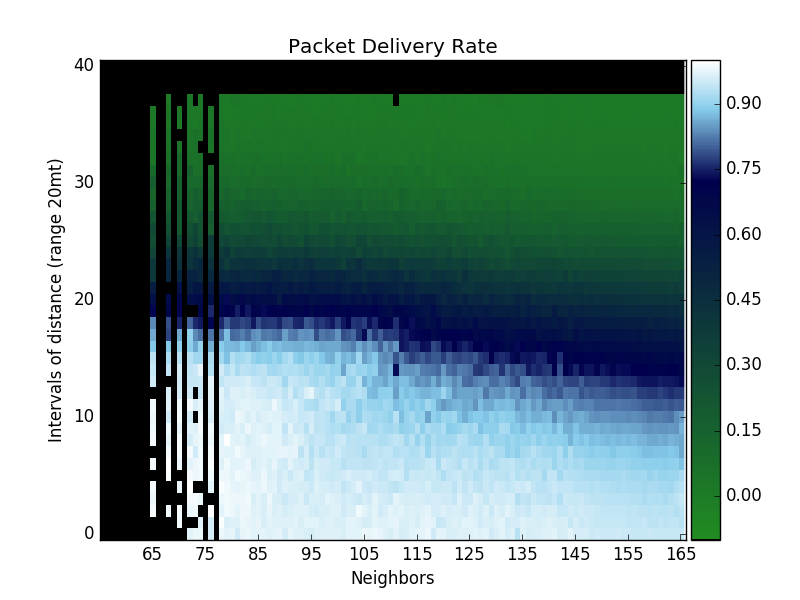
\includegraphics[width=0.8\textwidth]{fig/Original_test_640_plot.png}
    \caption{PDR of the original model in the evaluation.}
    \label{fig:pdro}
\end{figure}
\begin{figure}[H]
    \centering
    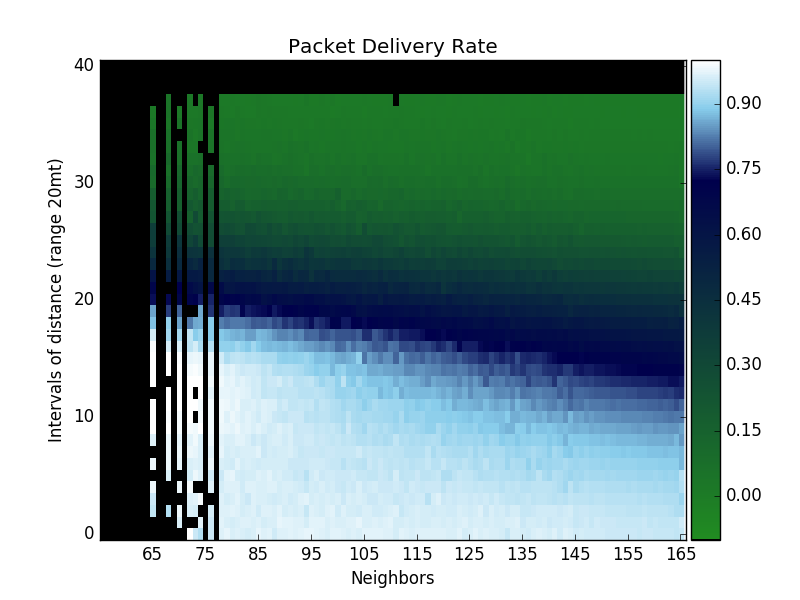
\includegraphics[width=0.8\textwidth]{fig/Markov_test_640_plot.png}
    \caption{PDR of the new model in the evaluation.}
    \label{fig:pdrn}
\end{figure}
\newpage
\subsection{Results}
\label{sec:Resultaccuracy}
\Cref{fig:pdro} and \Cref{fig:pdrn} show the PDR of the two model. As can be seen the two models have very similar results. The probability of correctly receives a packet decrease with the increasing of the neighbors and the distance.\\
As expected, a pair of vehicles that are very close have a very high probability of correctly receive a packet even if the receiver has an high number of neighbors.\\
\begin{table}[H]
    \centering
    {\tabulinesep=2.2mm
    \begin{tabu}{|l |l |l|}
        \hline
        $\mu$ & $|\mu|$ & $\sigma^2$  \\
        \hline
        $0.19\%$ & $2.53\%$ & $11.62\%$ \\
        \hline
    \end{tabu}}
    \caption{Result of accuracy measurement}
    \label{tab:accuracy}
\end{table}
As can be seen from \Cref{tab:accuracy} the results of the accuracy measurement, the two models have similar results. The result of the sample mean indicates that the original model correctly decoded in average $0.19\%$ packets more than the new model.\\
While the absolute value of the mean indicates that the original model decoded differently the $2.53\%$ of the packet with respect to the new model.\\
The standard deviation finally, indicates that there is a deviation of $11.62\%$ from the sample mean.
\newpage
